\documentclass[crop]{standalone}
\usepackage{tikz}
\usetikzlibrary{backgrounds}
\usetikzlibrary{trees,positioning,arrows}
\begin{document}
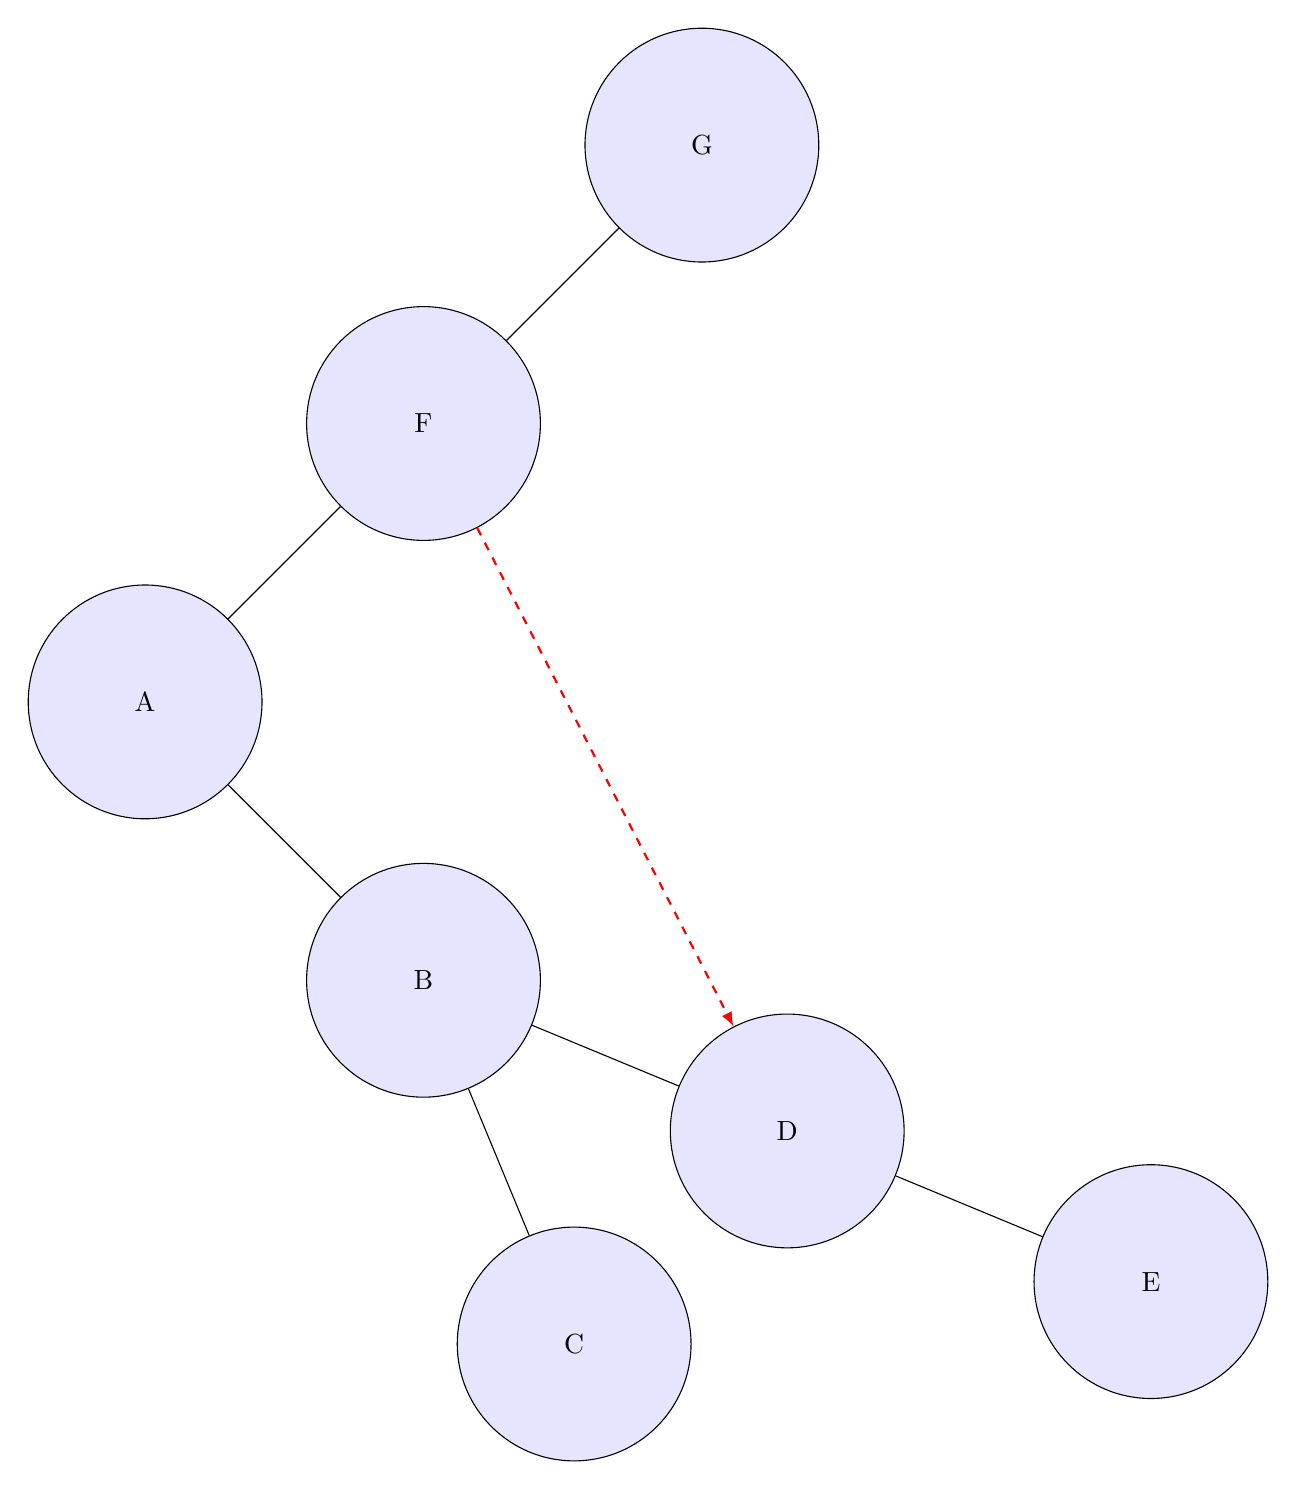
\begin{tikzpicture}[grow cyclic, text width=2.7cm, align = flush center,
every node/.style={circle,draw,fill=blue!10},
edge from parent/.style={black,thin,draw},
level 1/.style={level distance=5cm,sibling angle = 90},
level 2/.style={level distance=5cm,sibling angle = 45}]
\node {A} 
	child {node {B}
   	child {node {C} }  
	child {node (D) {D}  child{node{E}}}} 
	child {node (F) {F}
	child {node {G}}
		   };
		   \draw[->,dashed,>=latex,thick,red] (F) -- (D);
\end{tikzpicture}
\end{document}
